\documentclass{article}
\usepackage[utf8]{inputenc}
\usepackage{bbold}
\usepackage{graphicx}

\title{Modularity and random walks}
\author{Tom Burns @tfburns}
\date{20 May 2020}

\begin{document}

\maketitle

In response to Thomas Varley @ThosVarley, who tweeted on 20 May 2020: ``Has any mathematical work been done relating the modularity of a network to the distribution of the number of times a random walker will visit every node?  My intuition says that if the distribution is narrow, the network shouldn't be modular. I'm not sure, though."

These (informal) notes show why this intuition is false.

\paragraph{Fact 1: Complete graphs have a one-point probability distribution of vertex visitations in a random walk.}
Let $K_n$ be a complete graph, where $n \in \mathbb{N}$ is the number of vertices. Let us say that a random walk starts on an arbitrary vertex and may `visit' another vertex in the graph iff those vertices share an edge, and let all possible visits be equally likely. In a random walk on $K_n$, at a timestep $t$ in the random walk the probability of being located at a vertex $k$ at timestep $t+1$ is $1/n$, since in the complete graph all vertices are connected and in a random walk all edge transitions are equally likely. The distribution of vertex visitation probabilities is therefore a one-point distribution and infinitesimally narrow. It is a stationary stochastic process.

\paragraph{Corollary 1: A vertex's visitation probability in a random walk on a graph is proportional to its degree.}

\paragraph{Fact 2: It is possible to construct an infinitely modular graph with a two-point probability distribution of vertex visitations in a random walk.}

Let $K_n$ be a complete graph, where $n \in \mathbb{N}$ is the number of vertices. By fact 1, at a timestep $t$ in the random walk on $K_n$ the probability of being located at a vertex $k$ at timestep $t+1$ is $1/n$. Let $G$ be a graph which we construct by connecting two complete graphs of the same size with a single edge between an arbitrary vertex in each graph. This will maintain the degree of all but one of the original vertices in each of the complete sub-graphs, whereas the degree of the vertices which connect the complete sub-graphs increase their degree by 1. By induction, we may continue connecting additional complete graphs of the same size while guaranteeing all vertices in $G$ have a degree of $n-1$ (if they do not connect two complete sub-graphs) or $n$ (if they connect two complete sub-graphs). By corollary 1, we have a two-point probability distribution of vertex visitations in a random walk.

Let a metric for graph modularity be the number of connected components, where we define a component to be any subgraph which can become disconnected by cutting a single edge. Let us say a graph has $N$-components if it has $N-1$ such edges. By the method above, we may construct $G$ to have as many connected components as we wish, and thus be infinitely modular while maintaining a two-point probability distribution of vertex visitations in a random walk. Note: Although these arguments hold for $n=1$ and $n=2$, it is more natural to see this in the case of $n\geq3$. The figure below shows the example of $n=5$ and N=3.

\begin{center}
    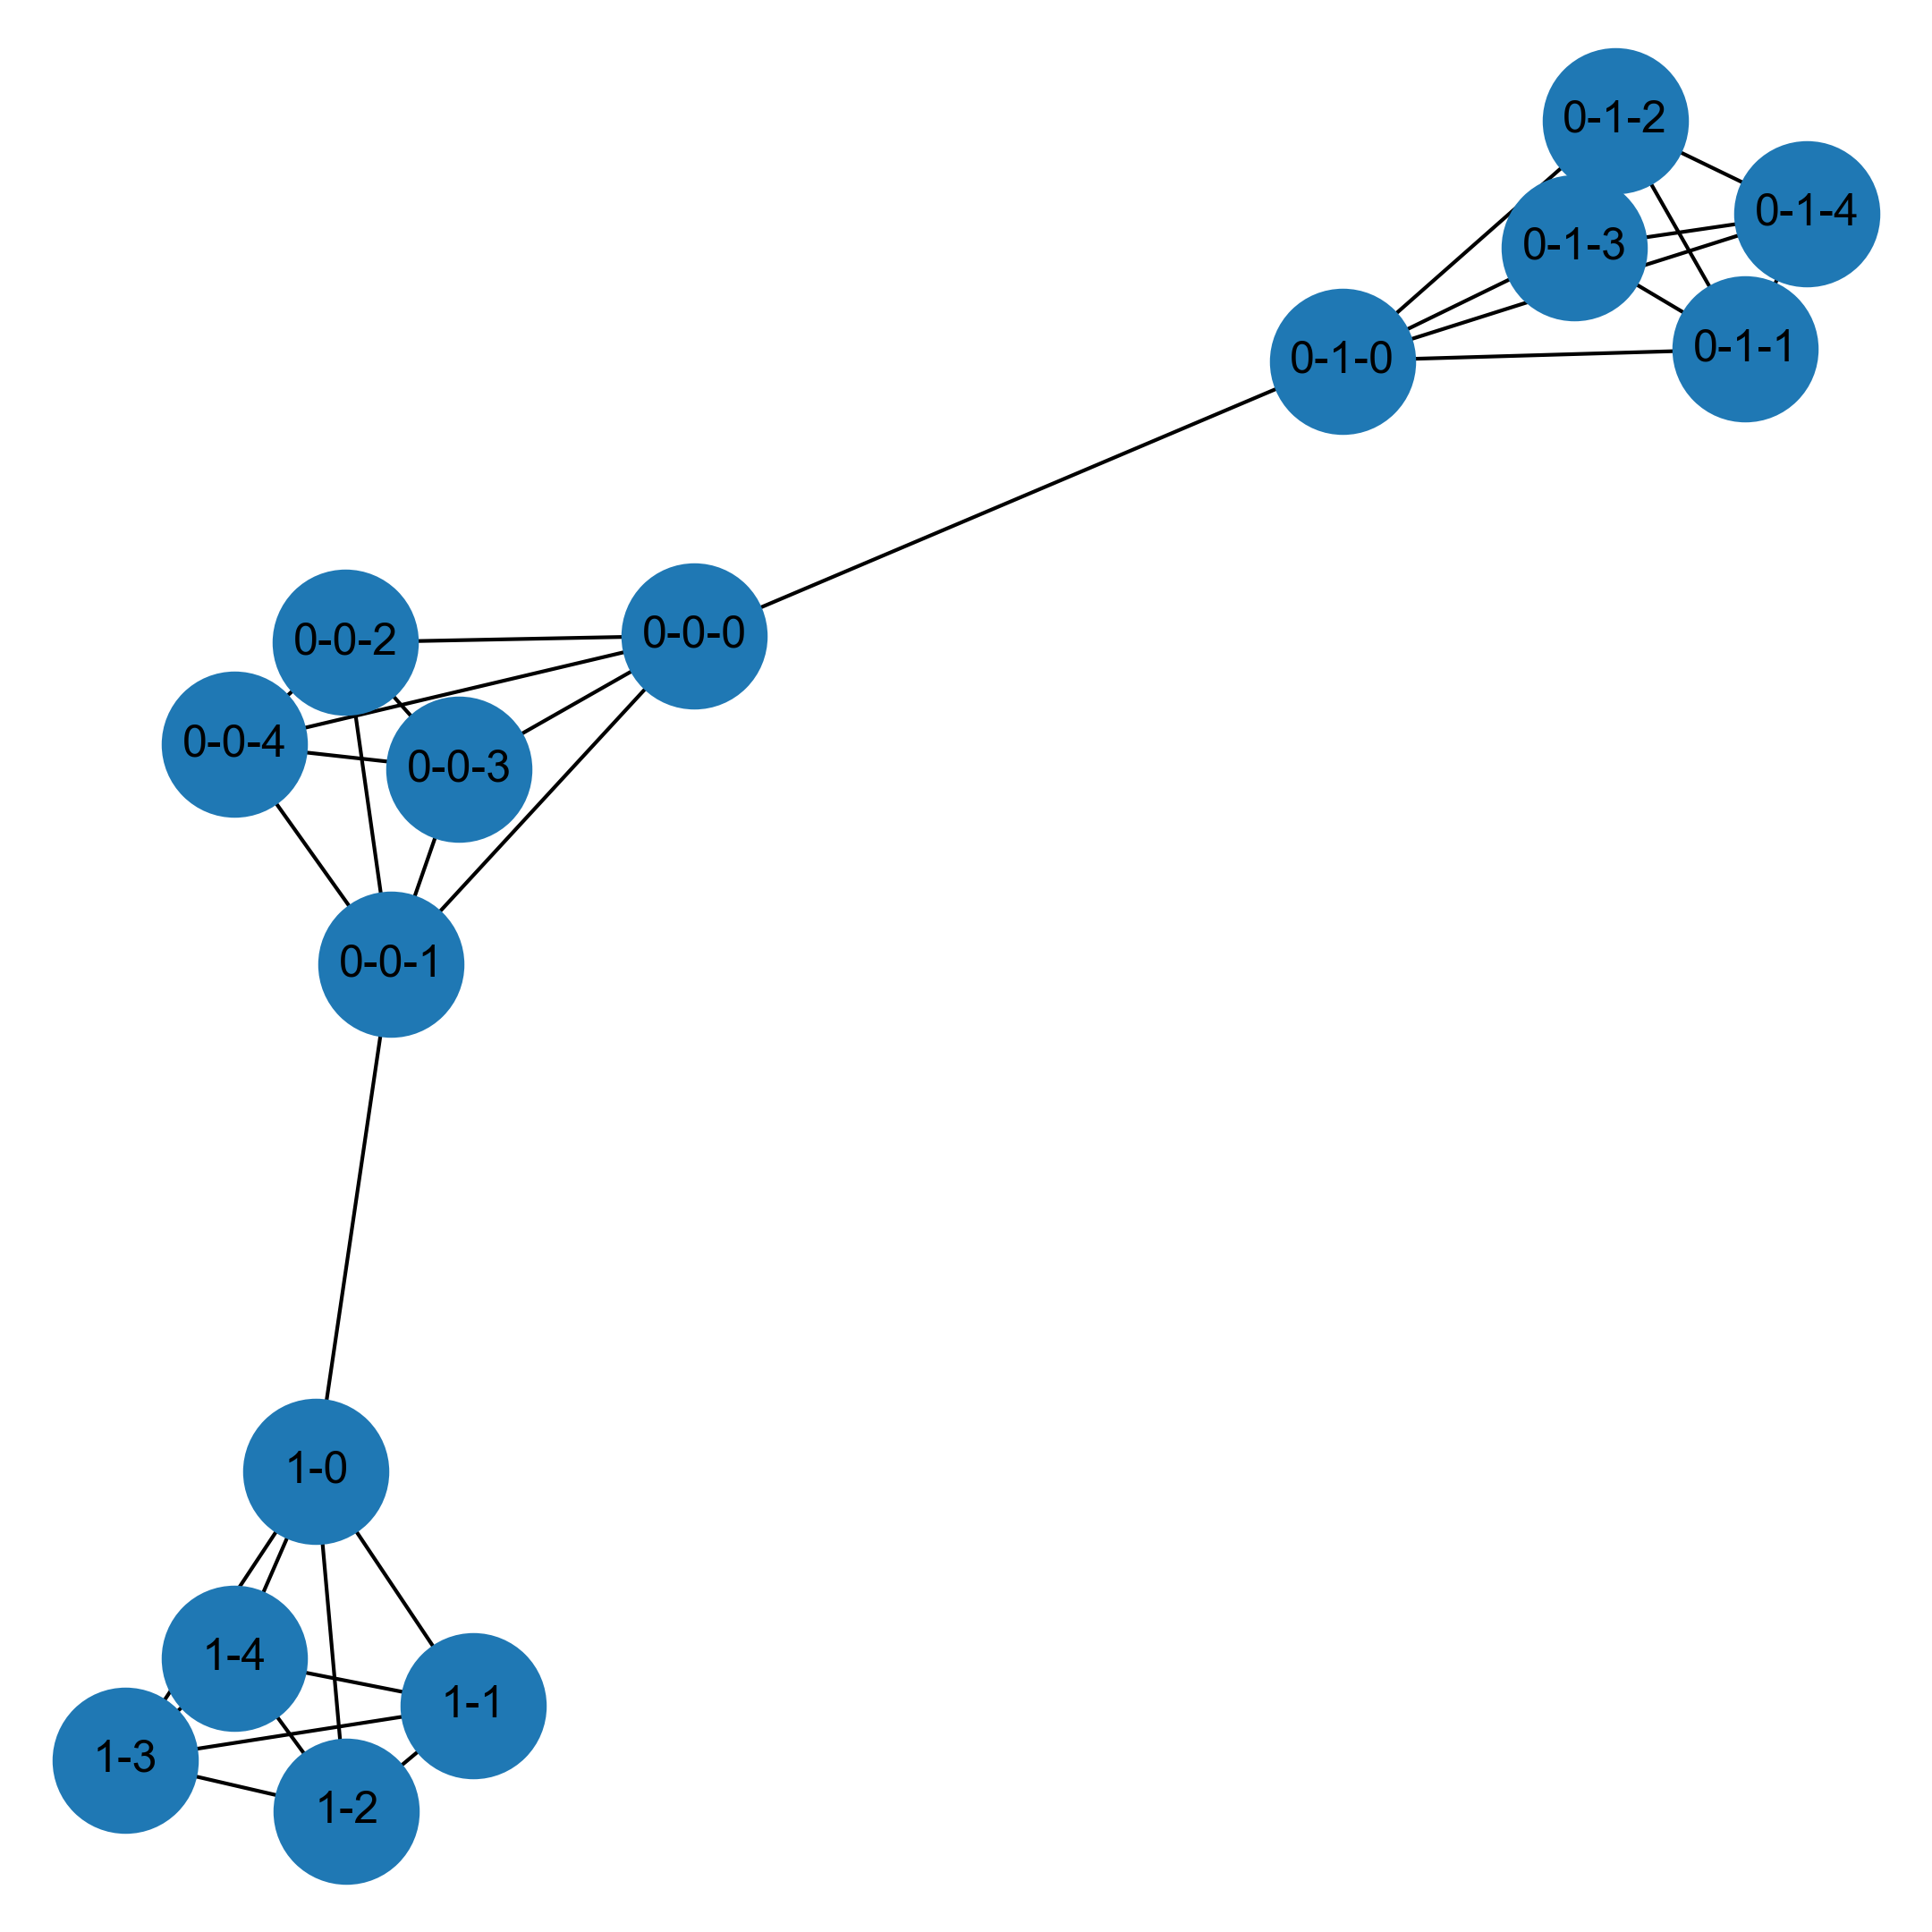
\includegraphics[width=6.5cm]{K5_K5_K5.png}
    \\
    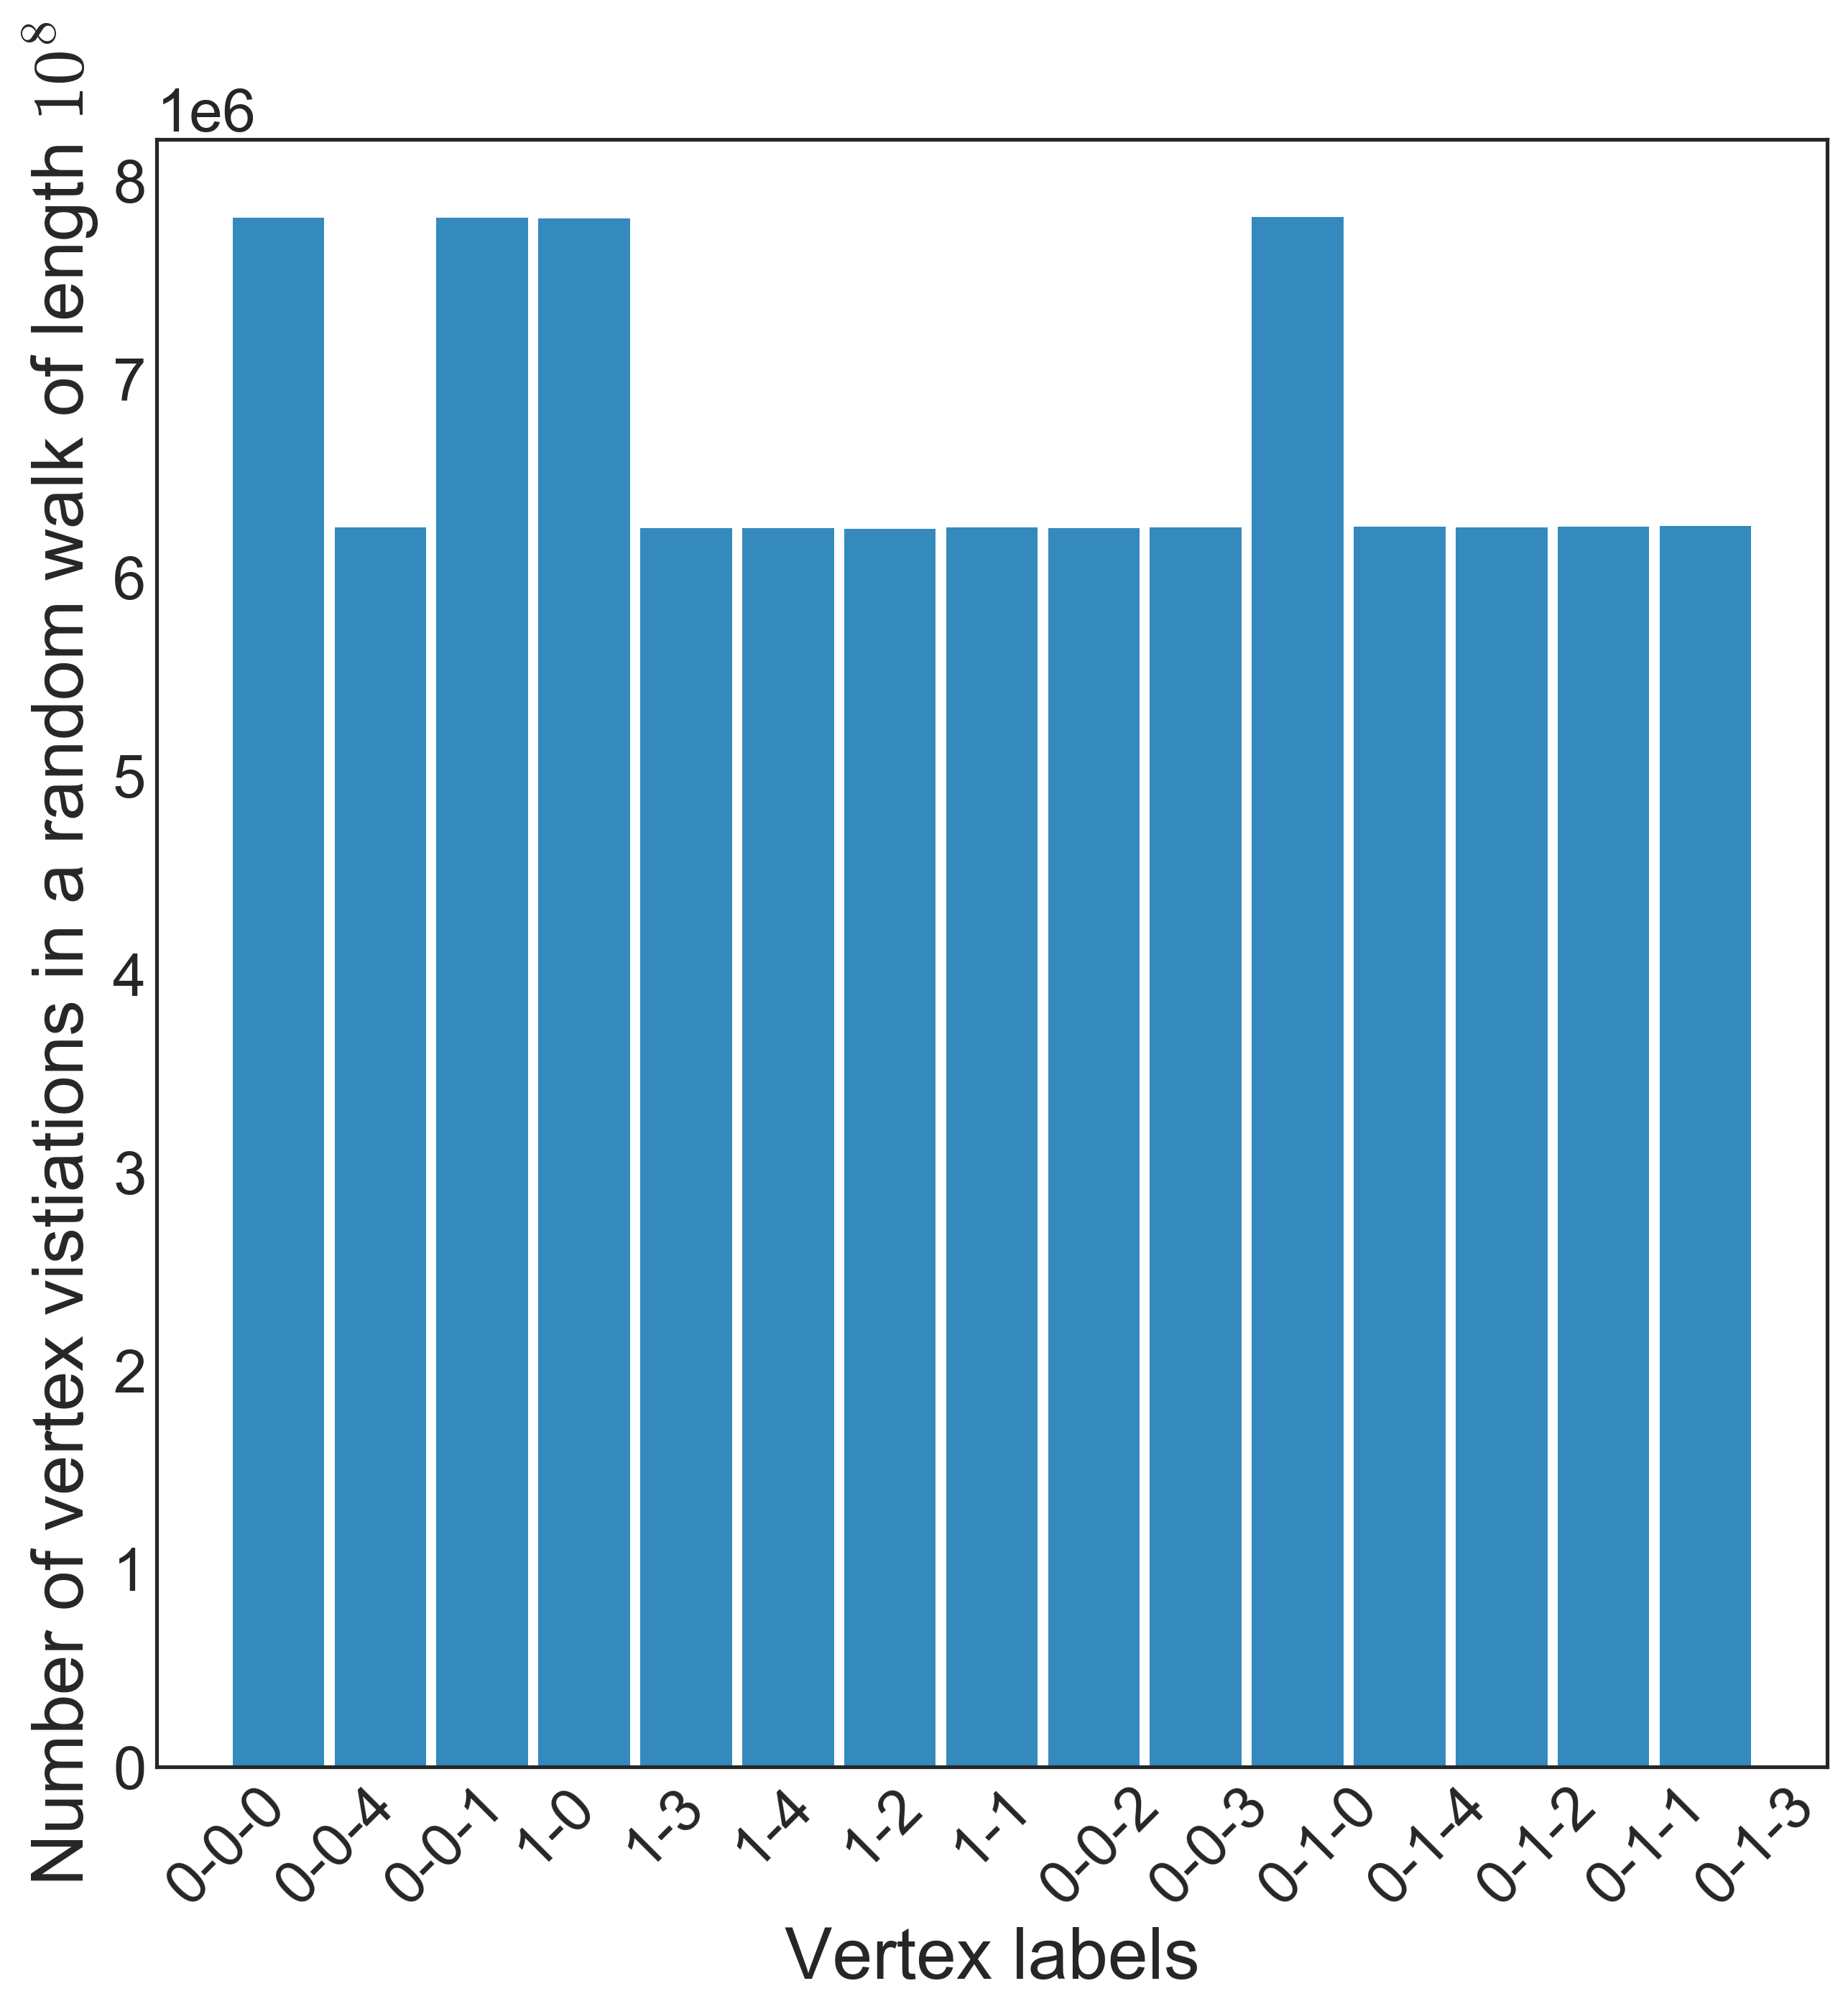
\includegraphics[width=6.5cm]{K5_K5_K5_dist.png}
    \\
    Simulated in Python. Code available at: https://github.com/tfburns/Graph-Gang/tree/master/notes/modularity-and-random-walks
\end{center}

\end{document}
